% This LaTeX 2e Class file is for the preparation of proposals for
% the NASA NSPIRES process.  Updated May 2015.

%\documentclass[preprint,12pt,authoryear]{elsarticle}
\documentclass[12pt,oneside]{article}

% \usepackage[dvips,draft]{graphicx}
\usepackage{graphicx}
\usepackage{natbib}
\usepackage[nolist,nohyperlinks]{acronym}
\usepackage{times}
\usepackage{fancyhdr}
\usepackage[small,compact]{titlesec}
\usepackage{url}
\usepackage{authblk}
\usepackage{amsmath}
\usepackage[pdftex,colorlinks=true,urlcolor=blue,citecolor=black,linkcolor=black]{hyperref}

% We use \sloppy to suppress word division and permit larger interword
% spacing so that lines are broken between words.
\sloppy

%%---------------------------- Global Settings ------------------------

%% Single-spaced+
%\renewcommand{\baselinestretch}{1.1}


%% Set margins for the bulk of the proposal.
\setlength{\topmargin}{0in}			% = 1in because LaTeX adds 1in
\setlength{\headheight}{0in}		% Height of page numbers
\setlength{\headsep}{0in}			% Distance from top of pagenum to text.
% \addtolength{\headsep}{-\headheight}% Adjustment for height of pagenumber.
\setlength{\topskip}{12pt}			% This is the height of the text.
\setlength{\footskip}{24pt}		% ???
\setlength{\oddsidemargin}{0in}		% = 1.5in because LaTeX adds 1in
\setlength{\evensidemargin}{0in}	% = 1in because LaTeX adds 1in

\setlength{\textheight}{9in}
\setlength{\textwidth}{6.5in}

%% Page decorations
\pagestyle{plain}
% \pagestyle{fancy}

% Decorations for most pages
\renewcommand{\headrulewidth}{0pt}
\fancyhead{}
\lfoot{}
\cfoot{\thepage}
\rfoot{\today}

% Decorations for the title page
\fancypagestyle{empty}{%
\fancyhf{} %clear all header and footer fields
\lfoot{}
\rfoot{\today}}

% Decorations for plain pages that begin chapters, etc.
\fancypagestyle{plain}{%
\fancyhf{} %clear all header and footer fields
\lfoot{}
\cfoot{\thepage}
\rfoot{\today}}


% Giving a new \contents name allows for putting a kind of title on
% the table of contents page.
\renewcommand*{\contentsname}{Photoclinometry for Improved Digital \\ Terrain Models}

% Short Title:
%          1         2         3         4         5
% 12345678901234567890123456789012345678901234567890
% Aqueous flow under Mars P, T, and atm conditions

% Change the way that \section numbers are displayed
\renewcommand{\thesection}{\arabic{section}}

% We want the bibliography section to be entitled "References"
\renewcommand*{\bibname}{References}

% This specifies the punctuation in citations within the text.
\bibpunct{(}{)}{;}{a}{}{,}

\setlength{\bibsep}{2pt}


\begin{document}

\title{Multi-view shape-from-shading for planetary images with
   challenging illumination}

 \author[1]{\rm Oleg Alexandrov}
 \author[1,2]{\rm Ross A. Beyer}
 \affil[1]{NASA Ames Research Center, Mail Stop 269-3, Moffett Field, CA
   94035, USA\\
  \{oleg.alexandrov,ross.a.beyer\}@nasa.gov
  }

 \affil[2]{Sagan Center, SETI Institute, 189 Bernardo Ave., Suite 100,
   Mountain View, CA 94043, USA}


% // {\it oleg.alexandrov@nasa.gov}
% \\
%  {\it ross.a.beyer.nasa.gov}
\maketitle

\begin{acronym}
\acro{ASP}{Ames Stereo Pipeline}
\acro{ISIS}{Integrated Software for Imagers and Spectrometers}
\acro{PDS}{Planetary Data System}
\acro{PSD}{Planetary Sciences Division}
\acro{USGS}{United States Geological Survey}
\end{acronym}

\begin{abstract}
  We propose and validate an algorithm for shape-from-shading that works
  for planetary data, with multiple input images, realistic camera
  models, non-Lambertian reflectance, variable albedo, uncertain camera
  positions and orientations, low angles of illumination, shadows, and
  occlusions. The algorithm uses stereo or other sources (such as LIDAR)
  to create an initial terrain model which is then optimized. We show
  that shape-from-shading is able to recover more detail than
  obtained from stereo, while eliminating stereo numerical artifacts and
  improving the terrain accuracy. Our implementation is released as
  open-source software as part of the NASA Ames Stereo Pipeline.
\end{abstract}

{\bf Keywords:} Shape-from-shading, photoclinometry, stereogrammetry,
surface reconstruction, terrain model.

\section{Introduction}

Shape-from-shading (SfS), also known as photoclinometry, is a set of
techniques for recovering surface relief based on variation in light
intensity recorded in images. It is based on the observation that the
brightness of a surface point depends on the angle between the incident
light ray and the surface normal (and in some models also on the
location of the observer), which, given knowledge of the position of the
light source and camera information, can be used to infer terrain slopes,
and by integration, the shape of the terrain itself.

In this paper we are interested in applying shape-from-shading to
recover high quality terrains from satellite images. We start from
initial guess terrain, that can be obtained either using
stereogrammetry, LIDAR data (examples can be LOLA or MOLA tracks,
appropriately gridded), or a terrain at a constant height. Shape-from-shading
is then used to refine this terrain.

We consider realistic camera models, such as pinhole and pushbroom,
rather than just an orthographic projection used in many publications,
multiple input images, each with its own exposure value, and
terrain-dependent albedo. We model and mitigate the fact that satellite
cameras can have have significant errors in position and orientation,
which we rectify by using bundle adjustment (with automatically
or manually picked interest points), varying the extrinsic parameters of
the cameras as part of the optimization, and solving the problem using
a coarse-to-fine terrain reconstruction approach.  We also study the
Lambertian, Lunar-Lambertian, and Hapke reflectance models, and we use
an approach in which the reflectance model is treated as a black box, so
the software can easily adapt to any such model. The parameters of a given model
can be set to different values on input, and, if desired, also optimized
as part of the problem. 

We are interested primarily, but not exclusively, in reconstructing
terrain on the Moon, towards the South Pole, due to recent interest in missions
there motivated by findings that craters that are permanently occluded
from the Sun may harbor water. At such locations the Sun is low in
sky, creating deep shadows that appear completely black. Our approach is
able to handle such difficult images by excluding from computation
pixels in the shadow, and handling gracefully areas where none of the
input images have information. We also model the fact that some terrain points are
occluded from the Sun, at which the terrain reflectance should be set to zero,
rather than being computed according to the reflectance model. We assume however that
the observing cameras are sufficiently high in the sky that no terrain
points are occluded from the cameras (the latter could easily be modeled
as well, as detailed in the text).

We validate our approach using images from the Lunar Reconnaissance
Orbiter Narrow Angle Camera (LRO NAC) \cite{robinson2010lunar}. These
images have a resolution on the order of 1 m/pixel.  In the first
approach, we create an initial guess terrain using stereo with images
artificially resampled by a factor of 10 from the originals, and run SfS
to improve this terrain using the same coarse images. We compare the
obtained terrain models before and after SfS with the ``ground truth''
terrain obtained from stereo at full resolution.  Alternatively, we ran
SfS on full-resolution LRO NAC imagery, and used the independently
acquired sparse Lunar Orbiter Laser Altimeter (LOLA) dataset
\cite{smith2010initial} for validation.  We show that with both
approaches SfS adds a wealth of new detail and improves the terrain
accuracy.

Our SfS implementation is released as a software program as part of the
NASA Ames Stereo Pipeline, a collection of open-source software for
stereogrammetry and geodesy, available under the Apache 2.0 license
(\url{http://ti.arc.nasa.gov/tech/asr/intelligent-robotics/ngt/stereo/}). The
program works with USGS ISIS camera models, which is the standard for
NASA planetary missions. The SfS tool has detailed documentation and
usage examples, with pre-compiled binaries for Linux and OSX.

\section{Comparison With Related Work}
\label{comp}


Shape-from-shading has a long history, starting perhaps with
\citep{van1951photometric}, who, based on variations in brightness on
lunar maria near the terminator, manually derived slopes of ridges.
The first paper that used a computer to do the calculations is perhaps
\citep{rindfleisch1966photometric}. Another notable early paper is \cite{Kirk:1977fk}.


A widely cited review of shape-from-shading methods is
\cite{zhang1999shape}, that divides the SfS approaches into four
categories: minimization approaches \cite{ikeuchi1981numerical},
propagation approaches \cite{horn1970shape}, local approaches
\cite{pentland1984local} and \cite{lee1985improved}, and linear approaches
\cite{pentland1989shape} and \cite{tsai1992fast}, with the latter two
methods using strong approximations of the problem.

Minimization methods are what is favored in the literature, due to their
generality and versatility, such as being able to model many aspects of
the problem, and ease of implementation. This is what we use in this
paper.

Our cost function has three components, the first two corresponding to brightness and
smoothness constraints, following \cite{ikeuchi1981numerical},
\cite{horn1990height}, \cite{lee1993shape}, etc. We also have a third constraint,
which tries to keep the terrain being optimized not too far from the initial guess. 
These and many other
works solve the problem in two steps, by first minimizing a cost
function to find the surface normals, then minimizing a second cost
function to recover the surface height from the normals (the integration
step).  For simplicity, we solve for the surface height directly, with
the surface normals computed from it during optimization as needed. A
discussion of these two approaches is in
\cite{crouzil2003multiresolution}.

To improve the speed of convergence, avoid local minima, and handle
errors in camera positions and orientations, we solve for the unknown
terrain (and also for albedo, image exposures, and cameras) using a
multi-resolution approach, \cite{terzopoulos1984efficient},
\cite{crouzil2003multiresolution}.

We recover the shape from multiple images. This has been done before by
many authors. An example is \cite{wu2011high}, which, like us, uses
stereo as an initial guess. It assumes constant albedo, and Lambertian
reflectance, no shadows, and accurate camera information.  The thesis
\cite{lux2011multi} is in similar vein. It has an example for SfS
applied to asteroid reconstruction, but using the Lambertian model and
without comparison to measurements.

The paper \citet{lohse2006derivation} considers multi-image
shape-from-shading for the Moon. It uses the Lunar-Lambertian reflectance
model, image-dependent exposure, and it prepares the images by using
bundle-adjustment to reduce camera errors. It does not use a smoothness
penalty term which we found to be essential, and it does not do comparison with
measurements.

The work \cite{grumpe2011construction} is very intriguing. It does
multi-image shape from shading for the Moon, and it uses hyperspectral
images to infer the minerals on the surface and as consequence the
spatially variable surface albedo that can then be added as a known
quantity in the cost function. Their newer paper
\cite{grumpe2014construction} uses very coarse input DEMs (the LOLA
gridded DEM and the GLD100 DEM based on the Wide Angle Camera (WAC)
imager), whose resolutions are on the order of 100 m/pixel, and their
final results have an elevation error of about 30~m, while we start with
LRO NAC based DEMs whose height error is on the order of a few meters
and we further improve upon them with SfS.

\cite{herbort2011reconstruction} is concerned with fusing single-image
shape-from-shading with active range scanning for refining elevation
models. It considers non-Lambertian models and variable albedo. It uses
an interesting penalty term that enforces that the partial derivatives
of the blurred (hence low-passed) surface being optimized remain close
to the analogous quantity for the original surface.  This requires an
extra weight parameter that would need tuning.

The paper \cite{o2012new} does single-image shape-from-shading for Mars,
using the Lambertian and Oren-Nayar reflectance models, with pinhole
and push-broom camera models. There are no comparisons with measurements
shown. In \cite{tyler2014merged} a software tool to create terrain models for
the Moon and Mars using multi-view SfS is presented, though neither the
full paper nor the software is available to describe what it does in
detail. Also worth mentioning is \cite{capanna2013three}, it uses
maximum likelihood estimation to reduce sensitivity to noise, and was
applied to reconstructing the Lutetia asteroid. The paper
\cite{samaras2000variable} models multi-view shape-from-shading with
piecewise constant albedo with applications to face reconstruction.

A very related recent paper is \cite{wu2016shape}. They also do
shape-from-shading on the Moon, recovering both shape and albedo. Yet,
they use a single image, and constrain the problem using a much
lower-resolution DEM, and their results only show that visually things
look promising.

A mathematical analysis of the well-posedness of the multi-view SfS
problem is given in \cite{jin20083}.

\section{The Algorithm}

\subsection{The Cost Function}

We represent the terrain as a function $\phi(x, y),$ describing the heights
over a sphere. This is sufficient for planetary applications,
though not for irregular shapes like asteroids. We assume that we have
one or more views of this terrain from satellite images, for which we
also know the position of the illumination source (the Sun, which we
represent as a point), as well as the positions and orientations of the
cameras. The cost function to be minimized is
\begin{multline}\label{cost}
\int\!\! \int \! \sum_k \left[ I_k(\phi)(x, y) - T_k A(x, y)
 R_k(\phi)(x, y) \right]^2\,  \\
+ \mu \left\|\nabla^2 \phi(x, y) \right\|^2  
+ \lambda  \left[ \phi(x, y) - \phi_0(x, y) \right]^2
\, dx\, dy.
\end{multline}
It is made of three terms, with weights $\mu > 0$ and $\lambda > 0$
attached to the last two.

The first term is the brightness constraint. It enforces that the simulated light intensity
for the given terrain agrees well with the light intensity as acquired
by the camera. It is well-known that if we only use this constraint, the
photoclinometry problem is not well-posed \citet{horn1990height} and the
resulting terrain will not be physically meaningful. Hence the need for
the second constraint, usually called the smoothness constraint. It
enforces that the obtained terrain
be reasonably smooth, and the weight $\mu$ is used to control the
smoothness amount. The SfS solution is known to reveal high resolution
detail, yet it may drift at larger spatial scales \cite{grumpe2014construction}.
That is the reason for the third term, with the weight $\lambda,$ 
that keeps the solution close the initial guess $\phi_0.$ 

Here, $I_k(\phi)(x, y)$ is the $k$-th camera image interpolated at
pixels obtained by projecting into the camera 3D points from the terrain
$\phi(x, y)$, $T_k$ is the $k$-th image exposure, $A(x, y)$ is the
terrain-dependent albedo, $R_k(\phi)(x, y)$ is the reflectance computed
from the terrain for $k$-th image, and $\left\|\nabla^2 \phi(x, y) \right\|^2 $ is the sum
of squares of all second-order partial derivatives of $\phi.$

The variables of optimization are the terrain and albedo at each point
$(x, y)$, and the exposure, camera position, and camera orientation for
each image. We start with initial guesses for these parameters, and they
can be independently kept fixed or varied.

\subsection{The Reflectance Model}
\label{reflectance}

A key ingredient in the SfS problem is the reflectance model to be used, which describes
how a surface reflects light. The simplest model is the Lambertian,
$$
R(\phi)(x, y) = \cos(i)
$$
which states that the reflectance at a terrain point is only dependent
on the incidence angle $i$ (the angle between the illumination
direction and the surface normal at a terrain point). This model is
often insufficient, and many adjustments to it have been used.

For the Moon, we use the Lunar-Lambertian model
\citet{mcewen1991photometric}, more specifically as given in
\cite{lohse2006derivation} (equations (3) and (4)), which states that

$$
R(\phi)(x, y) = \Lambda(\alpha) \frac{2\cos (i)}{\cos(i) + \cos(e)}
 + \left(1-\Lambda(\alpha)\right) \cos(i)
$$
where $e$ is the emittance angle, that is the angle between the surface
normal to the terrain and the viewing direction), $\alpha$ is the phase
angle (the angle between the illumination and viewing directions), and
$$
\Lambda(\alpha) = 1.0 + A\alpha + B\alpha^2 + C\alpha^3
$$
with
$$
A = -0.019, \  B = 2.42\times 10^{-4}, \  C = -1.46 \times 10^{-6}.
$$
Notice that the reflectance formula lacks the albedo factor, that one we
already factored out, as seen in Equation (\ref{cost}).

We also experimented with the Hapke model. That is described in section 
\ref{mars}.

\subsection{Discretization}

We discretize this problem using the finite difference method, hence the
domain of computation is a gridded rectangular box, and the terrain heights and
albedo become matrices of numbers. Central differences are used to find
the partial derivatives and surface normals.

The values of the terrain heights and albedo at the boundary are 
kept fixed during optimization.

\subsection{Initialization}

We assume that the cameras have been calibrated, and have known
positions and orientations. Bundle adjustment is optionally used to
reduce the errors in camera position and orientation before running
SfS. A known position for the illumination point source is assumed as
well.

Stereo on two of the images is used to get an initial guess for the
terrain $\phi(x, y).$ We also tested our algorithm by starting
with a constant terrain. The results returned by SfS in a such case look
plausible but we did not quantify their accuracy. In principle,
an initial surface obtained by any other means would work as well.

The initial albedo $A(x, y)$ is set to 1 everywhere (hence
its scale is absorbed into the image exposure). Then, using the fact that
the image intensity equals the image exposure times albedo times
reflectance, we derive the initial camera exposure for image $k$ as:

$$
T_k = \frac{ \int\!\! \int \! I_k(\phi)(x, y) \,dx\,dy }{ \int\!\! \int \! R_k(\phi)(x, y) \,dx\,dy}.
$$

We found the smoothness weight $\mu$ to be dependent on the instrument
acquiring the images. Hence, for each set up several values of
this parameter should be tried (using say a few or just one of the
images for speed), and its value can be chosen depending on which
solution is closer to the ground truth or otherwise results in a terrain
of satisfactory appearance, that is, a hillshaded image of this terrain
appears rather similar to the input images, without much noise or
excessive blur. A value of $0.06$ to $0.12$ worked well in our experiments.
For $\lambda$ we used a value of $10^{-4}$, increasing it sometimes up to $10^{-3}.$

\subsection{Handling Errors In Camera Positions and Orientations}
\label{multires}

Often times, the positions and orientations of satellite cameras
are not known sufficiently accurately, for example the position may be off by tens of meters or more.
This results in the SfS algorithm converging to an incorrect local minimum. 

We implemented the well-established approach of
first solving the problem on coarser versions of the input images and
terrain, in fact a pyramid of such datasets is used, with a scale factor
of 2 between pyramid levels, and subsequently refining the obtained
terrain and albedo while carrying over the exposures and camera
positions and orientations obtained at the previous level. Larger errors
in cameras require more pyramid levels. Optionally, the first camera can
be kept fixed, to ensure that the terrain does not drift away.

In our experience this approach works well for moderate positioning errors but is not 
reliable when the errors are large. An alternative is to use bundle adjustment,
which explicitly solves for camera adjustments so that matching features in
all images correspond to the same ground landmark. This approach is highly 
reliable, but it depends on correctly identifying the same feature in multiple images.
Existing algorithms, such as SURF fail if the differences in illumination between
images are too drastic, such as the shadows being in completely opposite directions.

We chose to manually select matching features in the images, and then perform
bundle adjustment. Using about 4 features per image proved adequate, and hence
the amount of manual work was small. Since the input images may be from very different
perspectives, we found out that map-projecting them onto a terrain corrects for that
and makes it much easier to visually identify features, which are then projected
back into the original images/cameras before being used for bundle adjustment.

An alternative approach being used to correct for camera errors is to compare a 
camera image with an artificially created image obtained by hillshading a terrain
with the same Sun and camera information as the image itself and comparing the two.
We expect this would work reliably only if there are no large albedo variations,
as hillshading does not model that. 

\subsection{Shadow Threshold}
\label{shadow}

When using SfS on planetary bodies, shadows cannot be avoided, and the
problem is exacerbated towards the poles. Particularly on the Moon,
shadows appear almost completely black and noisy. Simply minimizing the
cost function (\ref{cost}) will result in shadowed areas being
interpreted as having very small image intensity, and hence it appears
that the rays emanating from the Sun hit the ground almost parallel to
it. This results in the optimized shadowed regions appearing to to
recede as viewed from the perspective of the Sun.

This behavior is not in fact physically meaningless, in reality areas
not illuminated by the Sun \textit{must} indeed be lower in elevation
than the illuminated areas that are occluding the shadowed terrain.
However, for added precision, if say two out of three images of a given
area have valid pixels, while the third exhibits only shadows, the
latter's contribution to the cost function must be ignored.

We accomplish this by marking image pixels as valid or invalid based on
a per-image shadow threshold. We have developed a GUI tool that allows
the user to interactively pick pixels in the shadow, with the shadow
threshold being the largest of the shadow pixel values selected so
far. The tool also highlights in a different color the portions of the
images that fall below the shadow threshold, making it possible to pick
further points and increase the shadow threshold until visual inspection
confirms that an adequate shadow threshold value was achieved. Using
shadow thresholds has resulted in a measurable, if not dramatic,
increase in accuracy.

\subsection{Occlusions From The Sun}

Shadows can manifest themselves in different ways as well. At a given
point on the terrain being optimized the projection of this point into
the camera image can result into an illuminated pixel, yet if a ray is
traced from this point towards the Sun it may go through some portion of
the current terrain. This suggests that an inconsistency is
present. Either the current point's height (above the spherical planet)
is too large and it should be pushed lower so that perhaps its
projection into the camera falls into the correct shadowed region, or
maybe the reverse must happen, the terrain region occluding this point
from the Sun must be lowered so that the ray going towards the Sun does not
intersect it. 

At such points we set the computed reflectance to zero (hence we ignore
the local reflectance computed using the normal). Since the measured
image intensity at the point (the value of the pixel obtained by
projecting the point in the camera) is positive, it results in a large
term in the cost function. To minimize it, the terrain point should have
to move to a location of lower measured image intensity. We have seen
some improvements in using this approach, but a more thorough study is
needed.

In this work we assume that a camera is sufficiently high in the sky
that it sees all terrain points. If this was not the case, a similar
approach could be used as when handling the shadows, by excluding the
contributions of such points from the cost function.

\subsection{The Optimization}

We use Google's Ceres solver \citet{agarwal2012ceres} to minimize the
cost function. Ceres is a highly versatile and very large-scale least
squares solver using the Levenberg-Marquardt algorithm. It automatically
computes partial derivatives numerically, creates a sparse matrix for
the problem which it inverts appropriately at each iteration, and it
handles properly situations when this matrix is singular or not
well-conditioned. All the user needs to do is to provide routines for computing
the terms in the cost function, as well as stopping
criteria. (Ceres is also able to prevent unreasonably large cost function
terms from dominating the computation, though we did not use this feature.)

\section{Results}

We tested our algorithm on Lunar images, both at low and high
latitudes, with one or more images, and with and without modeling
shadows.  We used data from the Lunar Reconnaissance Orbiter Narrow
Angle Camera (LRO NAC) from
\url{http://wms.lroc.asu.edu/lroc/search}. This sensor is a pushbroom
camera. The images come at about 1 m/pixel ground resolution. The
original datasets were converted to the USGS ISIS format, then we
performed radiometric calibration and echo correction before using them.
We also experimented with images from Mars and Charon (the satellite of Pluto).

\subsection{Single-Image SfS}
\label{single}

Here we use LRO NAC image M139939938LE that is at a latitude of about
$85^\circ$ South. To get an initial guess for SfS we created a terrain
model at 1 m/pixel (the image resolution) with the NASA Ames Stereo
Pipeline, pairing this image with the dataset M139946735RE. SfS was run
with the first image only.

The smoothness weight was set to $\mu=0.08,$ and we used
$\lambda=10^{-4},$ and the Lunar-Lambertian reflectance. The terrain
model is of size $456 \times 410$ pixels. The results are seen in Figure
\ref{fig:sfs1}.  Here we have no ground truth to compare against, but it
appears that the optimized terrain has a lot more detail without moving
too far.

\begin{figure}[h!]
\begin{center}
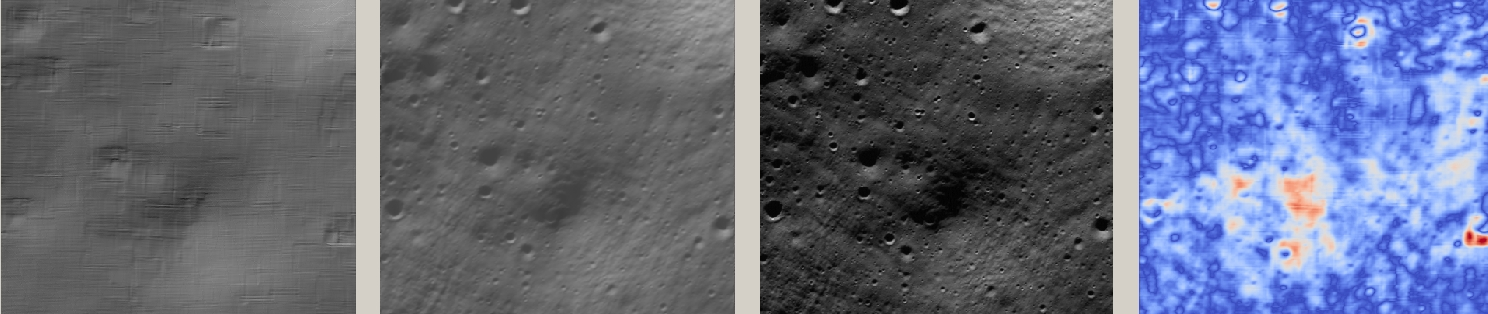
\includegraphics[width=6in]{figures/sfs1.jpg}
\caption[sfs]{Single-image SfS. The images are, from left to right, the
  initial hill-shaded terrain from stereo, the hill-shaded terrain obtained from
  SfS, the image used for SfS (draped over the initial terrain), and the
  absolute height difference of the initial and final terrains, where
  the brightest shade of red corresponds to a 2~m height
  difference.}
\label{fig:sfs1}
\end{center}
\end{figure}

It is important to note that the numerical artifacts seen in the
original terrain are not quite unexpected. Since the images are at 1
m/pixel, the terrain obtained from stereo has an effective
resolution on the order of about 5 m/pixel (since stereo matches
image patches rather than individual pixels) and here we rendered it at
1 m/pixel, so it is not unreasonable that stereo could not resolve
fine details and that noise jumps into view. 


For this example we did not vary the exposure of images, the albedo, or
the camera positions, as these would make the problem under-determined,
given that we have just one input image.  We also did not model shadows
and occlusions. It can be seen that small shadowed areas have been
handled rather gracefully.

\subsection{Multi-Image SfS At Low Latitudes}
\label{multiple}

\begin{figure}[h!]
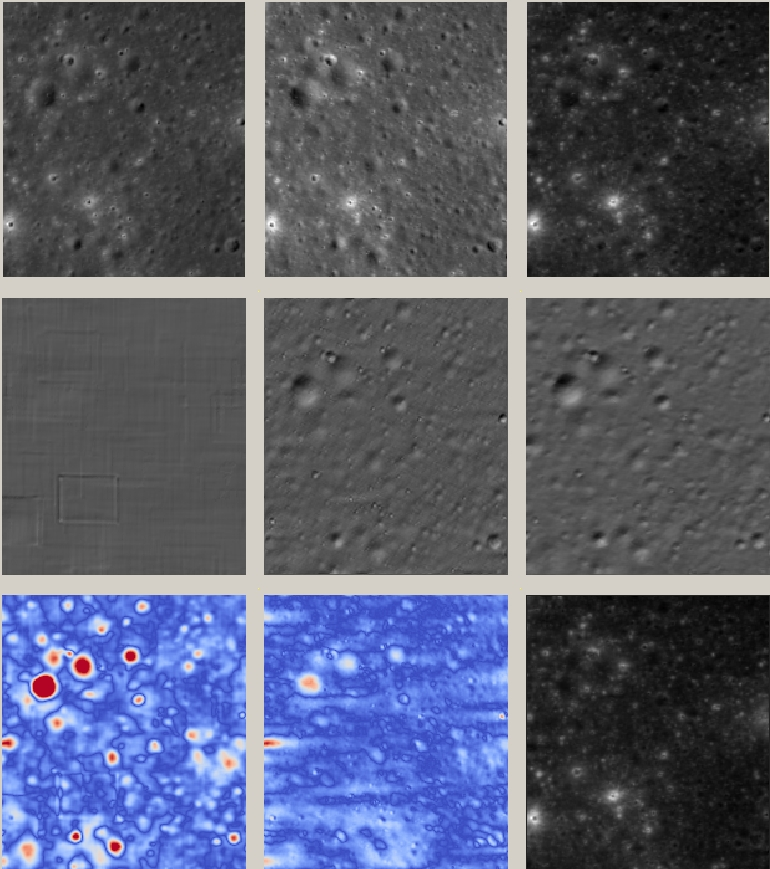
\includegraphics[width=6in]{figures/sfs2.jpg}
    \caption[Photoclinometry example]{
      \label{fig:sfs2} Multi-image SfS at low latitudes. Top row (left-to-right): original
      images, coarsened by a factor of 10, so at 10 m/pixel (draped
      onto the ground truth terrain). Middle row (left-to-right):
      Initial guess terrain at 10 m/pixel, the result of running
      shape-from-shading on these three images with the given initial
      guess, and the ``ground truth'' terrain. Bottom row: The absolute
      error between the initial guess to SfS and the ground truth, the absolute error
      between the SfS output and the ground truth (the brightest shade of
      red corresponds to a 10~m elevation error), and the optimized albedo.}
\end{figure}

Here we used LRO NAC images M1121224102LE, M1121209902LE, M1098830077LE, and M1149488705LE 
of a relatively flat region slightly above the Apollo 15
landing site (about $3.7^\circ$ East and $26^\circ$ North).

To correct for camera positioning errors we ran bundle adjustment on all
four images, with interest points picked manually, as the illumination
conditions were too different for the automated interest point
detection to work. 

To be able to estimate the accuracy of SfS, we purposefully
worked with images made coarser by a factor of 10 (hence at 10
m/pixel). We created an initial guess for SfS by running stereo on
the first two of these coarsened images, then we ran SfS with the first,
third, and fourth coarse images (the second image was sufficiently
similar to the first one that we thought it would not add much
information). We used the terrain obtained using stereo with the first
two original images at 1 m/pixel as ``ground truth'' for
validation (with the terrain heights binned to a 10 m/pixel grid to be
consistent with the SfS terrain). We applied a rigid alignment to the
``ground truth'' terrain to make it as close as possible to the coarse
terrain used as input to SfS.  And we investigated if SfS can make the
coarse terrain even closer to the ``ground truth''.

In this example we varied the terrain, albedo, and image exposures, and
used the Lunar-Lambertian model.  The terrain was on a grid of size
$196\times 223$ pixels. The smoothing weight $\mu$ was set to 0.08 and
the weight $\lambda$ constraining the solution close to the initial
guess was $10^{-4}$. After optimization, the mean error to the ``ground truth'' DEM went
down from 1.60~m to 1.02~m, while the standard deviation
decreased from 1.92~m to 0.93~m. The results are seen in Figure \ref{fig:sfs2}.

In this example we did not vary the camera positions and poses as part
of the optimization problem, since they were-predetermined using bundle adjustment. When trying
to doing to, the results were within a few centimeters of the above. 

\subsection{Multi-Image SfS At High Latitudes With Shadow Modeling}

\begin{figure}[h!]
\begin{center}
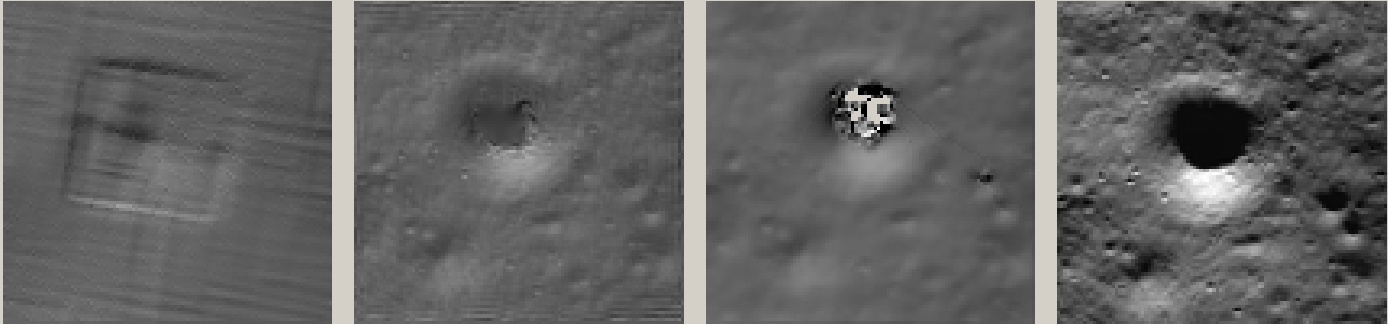
\includegraphics[width=6in]{figures/sfs3.jpg}
\caption[sfs]{Multi-image SfS at high latitudes. The images are, from
  left to right, the hill-shaded initial guess DEM for SfS, the hill-shaded DEM obtained
from SfS, the ``ground truth'' DEM, and the first of the
images used in SfS, draped onto the ground truth DEM.}
\label{fig:sfs3}
\end{center}
\end{figure}


Here, like in section \ref{single}, we worked at $85^\circ$ latitude
South on the Moon, and used the similarly looking images M139939938LE
and M139946735RE to run stereo. We also employed images M173004270LE,
M122270273LE, and M119922302RE, and we ran SfS on the first, third,
fourth, and fifth of these (the second image being rather similar to the
first should not add much additional information).

As in section \ref{multiple}, we used stereo with the original 1 m/pixel
images to create the ``ground truth'' terrain, while SfS was run with
images 10 times coarser. SfS was initialized using stereo from the same
coarse images. Validation was done as earlier as well.

As before, we performed bundle-adjustment with manually picked interest
points to reduce the initial camera errors, and then ran SfS without the
multi-resolution approach. Since large shadows are present, we used
shadow thresholds as described in section \ref{shadow}. We used the
Lunar-Lambertian model. The terrain being optimized was $102 \times 100$
pixels in size. We again varied the terrain, camera positions and
orientations, and image exposures. We did not float the albedo as there
were no obvious albedo variations. The smoothness weight was set to
$\mu=0.12$ and we used $\lambda=10^{-4}.$

As result of SfS, the mean error between the shape being optimized and
the ground truth decreased from 2.77~m to 1.52~m, while the standard
deviation decreased from 3.01~m to 2.12~m. 
The results are shown in Figure \ref{fig:sfs3}.

If the shadow thresholds are not
used, the mean error of the SfS terrain compared to the ground truth
is instead 1.54~m, and the standard deviation is 2.21~m. Hence, using
the shadow threshold does help, but the improvement is minor. This may have 
a larger effect on terrains where shadows are much more dominant. 

If using, as done earlier, shadow thresholds, but switching the model to the pure Lambertian, 
the mean and standard deviation of the error compared to the ground truth are, after SfS,
1.58~m and 2.21~m. We can see that, as expected, the Lunar-Lambertian performs
better than the Lambertian model. 

We also experimented with not varying the camera parameters as part of
the optimization problem, and the results became a little worse.  The
results are also somewhat worse if the albedo is floated. The insight
here is that floating the albedo should only be enabled if albedo
variations are obviously seen in the imagery, and it is perhaps
suggested to experiment with both floating and not floating it, as this
being a complex problem with imperfect reflectance modeling, it is not
clear beforehand which strategy will yield the best results.

\subsection{Large-Scale High-resolution SfS And Comparison With LOLA}
\label{lola}
\begin{figure}[h!]
\begin{center}
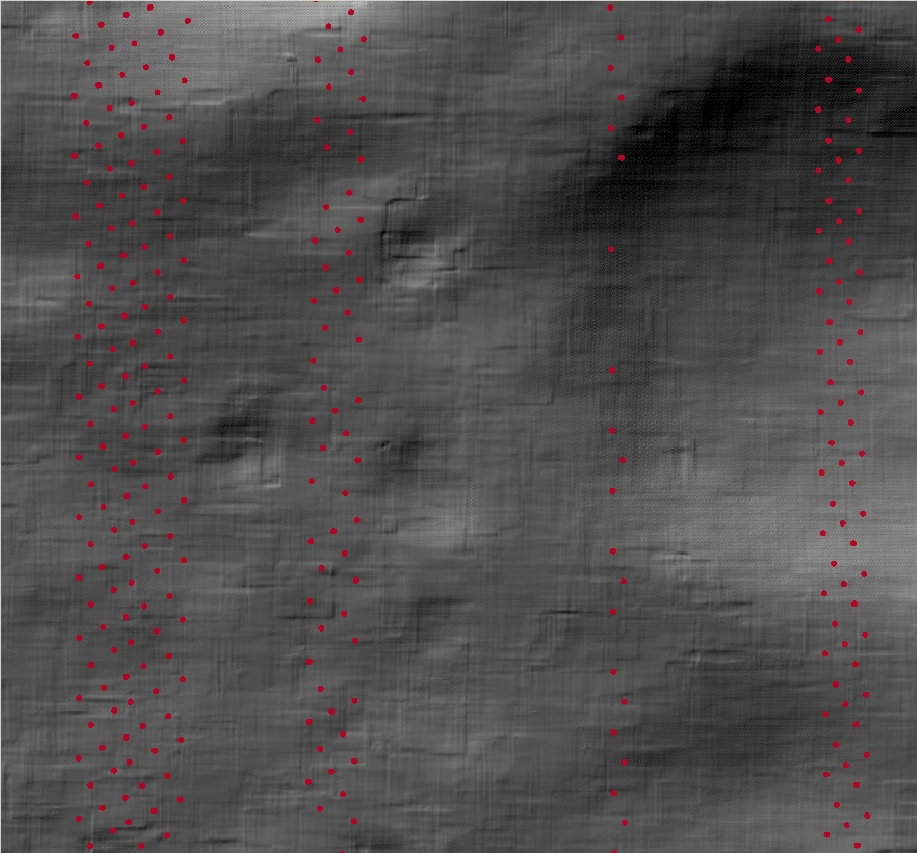
\includegraphics[width=3in]{figures/sfs_lola_before.jpg}
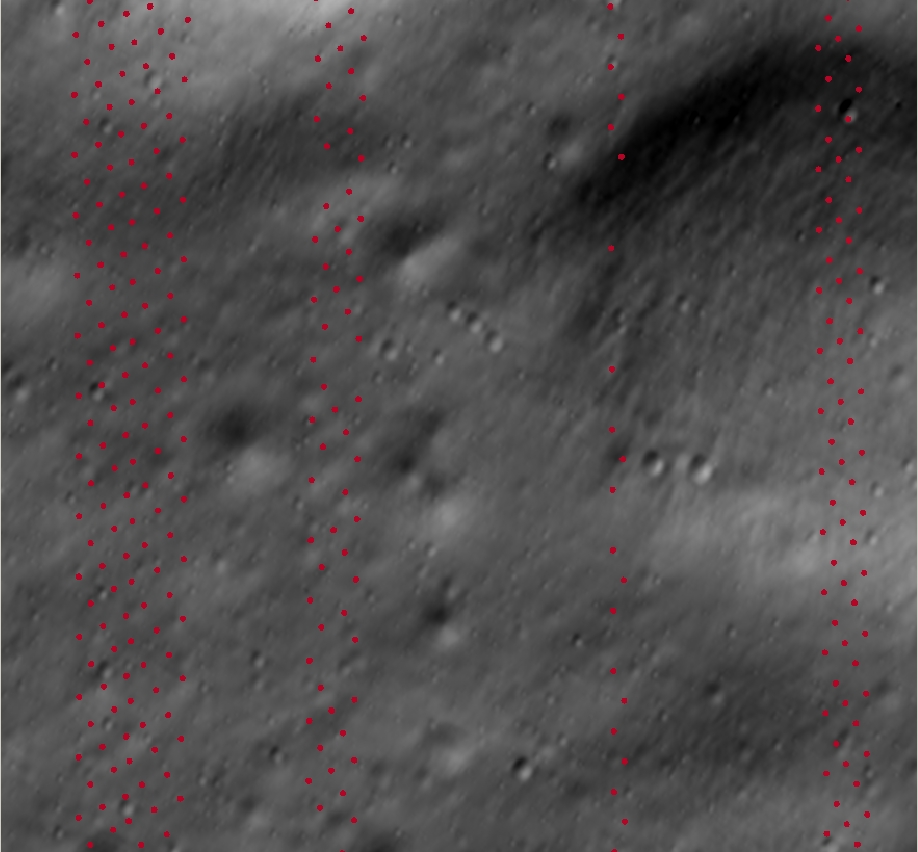
\includegraphics[width=3in]{figures/sfs_lola_after.jpg}
\caption[sfs]{A small portion of the terrain at 1 m/pixel, 
before SfS (left) and after SfS (right), with LOLA tracks super-imposed for illustration.}
\label{fig:sfslola}
\end{center}
\end{figure}
So far, we ran SfS mostly on small clips and on images at 1/10-th the original resolution,
reserving the terrain obtained from the original high-resolution images as
``ground truth''.  Here, we perform multi-image SfS using full-resolution imagery, and
validation with independently acquired ground truth, in the form of the
Lunar Orbiter Laser Altimeter (LOLA) dataset \cite{zuber2010lunar}. We
show that SfS can work on a large terrain, which requires
partitioning it, and different sets of images to be used for SfS for each
partition.  Hence we show that in principle SfS can scale to arbitrarily
large terrains given sufficient overlapping images from various
illumination conditions covering each portion that terrain.

LOLA is a dataset of height measurements on the lunar surface, consisting
of tracks that go North-to-South. The points in each track are separated by about 20~m,
and the distance between tracks is about 1.25 km at the equator, narrowing down 
towards the poles. The nominal vertical precision of each point is about 10 cm, but the actual error
is about 1~m (we discuss this further in the next section). Hence, this dataset is sparse, but it can still provide a measure of certainty that 
a terrain refined with SfS is more accurate (or at least no less inaccurate) than
the input terrain.

We selected a terrain around the Apollo 17 landing site ($30.8^\circ$
longitude and $20.2^\circ$ latitude) of size about $4.7 \times 4.2$ km,
and used a ground resolution of 1 m/pixel (the native LRO NAC
resolution). There was no single set of imagery of various illumination
conditions covering the entire terrain, so we partitioned it into two
overlapping regions (left and right region) and we used for SfS images
M134991788LE, M1142241002LE, and M162107606LE on the left region, and images
M104311715RE, M180966380LE, and M192753724LE on the right region. We
took care that the three images used each time are with the Sun being
positioned respectively reasonably left, right, and relatively high in
the sky, as evidenced by the pattern of shadows in each image. This
helps constrain the problem well and obtain more accurate results.

We first performed bundle-adjustment of all 7 images (the 6 images
mentioned earlier, as well as of M104318871RE, which together with
M104311715RE forms a stereo pair that was used to create the terrain for the
SfS initial guess) to eliminate camera alignment errors which would make SfS
inaccurate. Here we could not use the multi-resolution approach outlined
in section \ref{multires}, as the 7 images overlapped only in a very
narrow area. Automatic interest point detection failed, as illumination
conditions were too different, so we just picked manually features in
each of the images corresponding to the same set of landmarks on the
ground.

The two regions were still too large for SfS to work efficiently,
so they were further subdivided into tiles of about $300 \times 300$ pixels,
with a padding of 50 pixels for each tile (hence each tile was about 400 pixels in size).
The padding is needed to eliminate boundary artifacts when later the output SfS terrains are merged. We ran SfS on each tile
as multiple processes on a multi-core system, and then we mosaicked the obtained results.

To compare with LOLA, we brought the initial stereo terrain 
in alignment with LOLA and measured the discrepancy between the two, and
then repeated the same procedure with the SfS output terrain. 
The mean error to LOLA decreased from 1.40~m to 1.33~m, and the standard deviation of the error
went from 1.09~m to 1.03~m. The maximum error went from 17.3~m to 8.25~m. 
The terrain itself changed, as result of SfS, by a mean value of 0.33~m
with a standard deviation of 0.39~m. The results look reasonable given that the accuracy of
LOLA is 1 m/pixel. An illustration is shown in Figure \ref{fig:sfslola}.

In this case we did not float the albedo, and we used the
Lunar-Lambertian reflectance model.  Floating the albedo improve the
results by a very small amount. Using the Lambertian model makes the results somewhat worse, but still an improvement
from the initial guess to SfS.

We repeated the same experiment near the Apollo 16 landing site and for
two other datasets at $85^\circ$ longitude South. In each case the error
compared to LOLA went down after SfS, though not hugely so. For all
experiments we used the regularization term weight $\mu = 0.06$ and the
distance constraint weight $\lambda = 10^{-3}.$

As a final remark, we would like to note that in this experiment as
initial guess for SfS we used the terrain obtained from stereo of images
M104311715RE and M104318871RE. They covered entirely the area of
interest. For even larger terrains, it will need to be first partitioned
into areas sufficiently small that stereo can be performed on them,
before partitioning it further to run SfS as described earlier. The only
extra difficulty here would be that after stereo and SfS is run on each
portion, the optimized terrain regions need to be aligned to LOLA
individually, before being merged.

\subsection{Comparison With LOLA Using Reduced-Resolution Images}

While LOLA has a nominal ranging precision of 10~cm (that is, this is the measurement
error between the laser instrument and the point it hits on the ground), there exist uncertainties in 
determining the spacecraft position at any time. Overall, the global accuracy of the LOLA topographic
model is on the order of 1~m \cite{smith2011results}. Hence, it is not surprising that the results
from the previous section are, while a good sanity check, not a dramatic improvement.

To make the comparison with LOLA more relevant we need to study situations when the error
between stereo and LOLA is noticeably larger than the uncertainty in LOLA itself. For that purpose,
we took some of the earlier images (M104311715RE, M104318871RE, M180966380LE, and M192753724LE)
and added the image M113751661LE which has yet other illumination conditions. We resampled all images
by a factor of 4, hence the new images have an effective resolution of 4 m/pixel. We created
a stereo terrain from the first two images, then ran SfS on all images sans the second (which is
too similar to the first one). 

The stereo terrain was $434\times 456$ pixels and at a resolution of 4
m/pixel (hence covering a region of about 1.8~km in size). This
region intersected 7 North-to-South LOLA tracks and the ground had
sufficient topography variation (the standard deviation of the terrain
height was 16~m) that we felt confident aligning the terrain to
LOLA. After alignment to LOLA, the mean error between these two datasets
was 2.30~m with a standard deviation of 2.04~m. We ran SfS using the
Lunar-Lambertian model, floating the albedo and the cameras, with the
weights $\mu=0.06$ and $\lambda=2.5\times 10^{-4}.$ We aligned the
result of SfS to LOLA as well. The obtained mean error after SfS
compared to LOLA was 1.64~m and the standard deviation was 1.50~m, a
large improvement.

\subsection{SfS On Other Planets}
\label{mars}

\begin{figure}[h!]
\begin{center}
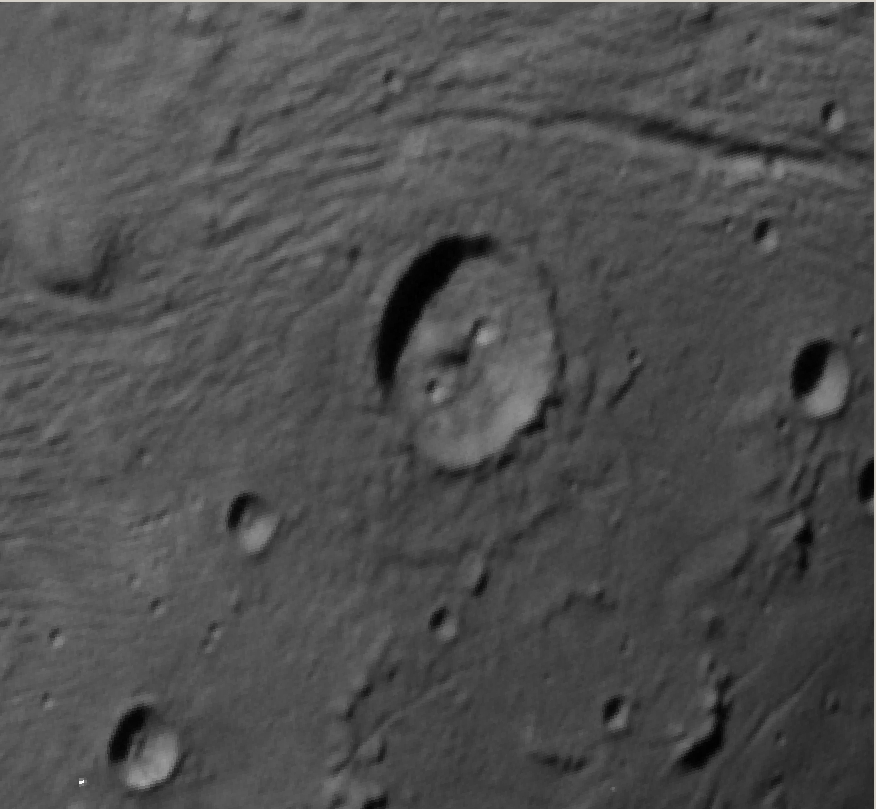
\includegraphics[width=3in]{figures/sfs_charon_img.jpg}
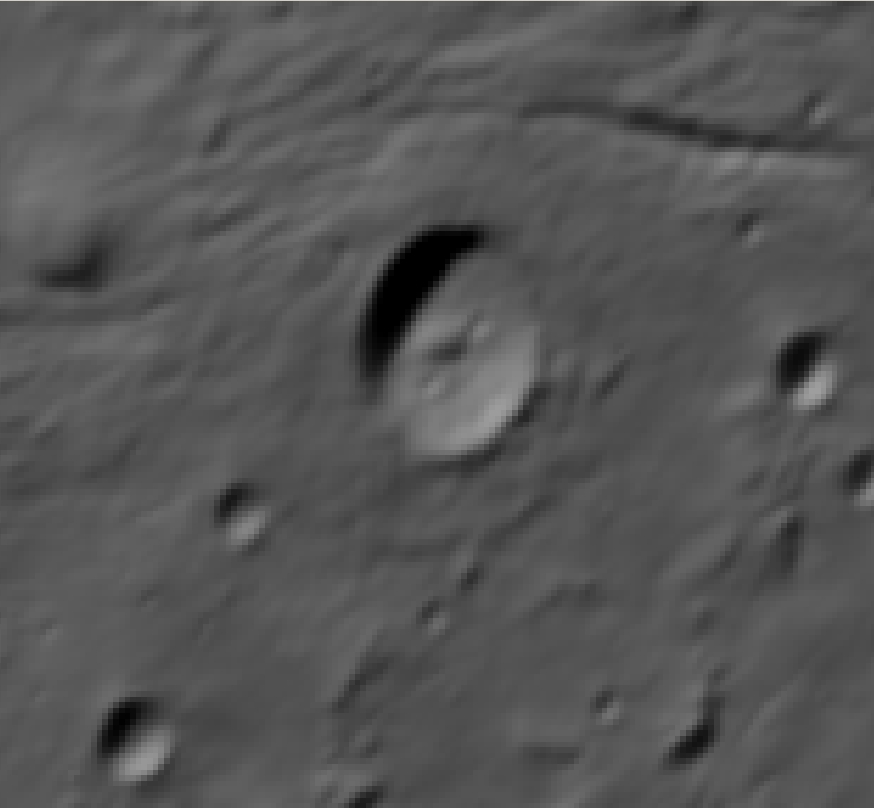
\includegraphics[width=3in]{figures/sfs_charon_dem.jpg}
\caption[sfs]{A portion of an image of Charon, at 400 m/pixel (left) and the computed hillshaded SfS DEM (right). The crater and elevated areas around it are clearly seen.}
\label{fig:sfscharon}
\end{center}
\end{figure}

We tried SfS on Mars with HiRISE images. A challenge with these images
is the fact that the solar incidence angle is relatively constant in all
of them. There is still some variation in illumination conditions due to
the fact that Mars has an axial tilt, so the position of the Sun in the
sky (and of the shadows on the ground) does vary somewhat with the
seasons. Yet the variation is little.

A ground truth dataset that can be used for validation is MOLA (Mars
Orbiter Laser Altimeter). This dataset is however much sparser than what
LOLA is for the Moon. Its nominal vertical accuracy is only on the order
of 1 m (compared with 0.1 m for the Moon), while HiRISE images are 0.25
m/pixel, and hence SfS with such images is expected to improve a terrain
by a small fraction of a meter. As such, MOLA is way too inaccurate and
too sparse to be used as ground truth. We chose to follow the same
validation process as earlier done on the Moon, using images resampled
at 1/10th of the original resolution for SfS, and then validate with
stereo terrain from the full resolution images.

Mars has an atmosphere, which gives rise to atmospheric scattering,
which we did not model, and a large variety of minerals on its surface,
and hence of ways in which it reflects light. The reflectance model used for 
Mars is usually the Hapke model \cite{hapke2008bidirectional}, \cite{hapke1993opposition}.
This model has 3 or 5 parameters $\omega, b, c,$ and then also $h$ and $B_0,$ 
if the opposition effect is also modeled. The values of these numbers vary considerably
depending on the specific site on Mars and the paper deriving them. We tried 
the various sets of values from \cite{johnson2006spectrophotometric} and \cite{fernando2013surface}.

We obtained the best results (defined as the smallest mean error between the
SfS-optimized terrain and the higher-resolution stereo-derived ground truth) using not the Hapke model,
but rather a variation of the Lunar-Lambertian model with different
values for the parameters $A, B, C$ compared to what we had on the Moon.
We believe our approach for Mars is still immature and more work is
needed. Particularly we should perform a deeper study of the
reflectance modeling, as well as modeling atmospheric effects. The lack of diversity 
in illumination conditions in the imagery (also for other Mars instruments) will continue to be an issue.

We also experimented with Charon, the moon of Pluto, using images from
the New Horizons flyby mission. Since this mission had a very short
window in which to acquire images, the illumination conditions are the
same in all of them. This is the reason why we believe using more than
one image (as opposed to just one) did not show any improvement in
surface detail after performing SfS. We got the best-looking results
using Lambertian reflectance. An illustration is shown in Figure
\ref{fig:sfscharon}.

\section{Conclusion And Future Work}

We implemented a shape-from-shading algorithm that models aspects of the
problem not often considered simultaneously in literature, such as
realistic camera models, multiple images, camera positioning errors,
variable albedo and image exposures, non-Lambertian reflectance, the
light source being low in the sky, shadows, and rigorous valuation with
ground truth. 

The SfS algorithm was shown to perform very well for Lunar images, both
at low and high latitudes. In each of our experiments we saw a wealth
of new detail after SfS, and the stereo artifacts were eliminated. We
estimated the accuracy of SfS in three different ways: comparison with
higher resolution dense terrain, comparison with the sparse LOLA dataset
when using 1 m/pixel imagery, and comparison with LOLA using 4 m/pixel
images. In each scenario we found that SfS improves the accuracy of the
terrain, within the limits of uncertainty of the ground truth we compare
to.

We showed that the algorithm can be run on a terrain that is too big to be
completely covered by a single set of images. We partitioned it
into smaller overlapping regions so that each of them is
covered by several satellite images of different illumination
conditions. Those regions can be further sub-divided into overlapping tiles,
and the tiles can be processed in parallel on single and multiple
machines taking advantage of multi-core and multi-machine setups
to greatly improve the runtime. The resulting SfS-optimized terrains can then be
seamlessly blended together. 

We observed in our experiments that, as expected, the Lunar-Lambert
reflectance model gives better results than the regular Lambertian for
the Moon. For Mars, we experimented with the Lambertian model as well as
with Hapke and a variation of the Lunar-Lambertian model with different
set of parameters.  We observed that SfS adds more detail for Mars
terrain, and the result may be more accurate as well for certain
reflectance models, but, as we expected, Mars is a much more difficult
planet than the Moon for SfS, both due to the less diverse illumination
conditions present in the imagery and because of very large variety in
terrain reflectance properties and the atmosphere. We also experimented
with Charon, Pluto's moon, obtaining visually satisfying results.

In the future, we would like to study in more detail the dependence and
accuracy of the shape-from-shading solution on the reflectance model
used, and try new reflectance models, such as Oren-Nayar and
BRDF models in general. It would be desirable to look into anisotropic
smoothing penalty terms, and a way to infer ways of automatically selecting the appropriate value of the
smoothing weight and the weight constraining the SfS terrain to the input terrain.

An interesting research direction is to impose geometric constraints,
such as explicitly enforcing that points observed to be in the shadow
are always guaranteed to be hidden from the Sun in respect to the
simulated terrain. Our modeling of occlusion is only a step in this
process.

\section{Acknowledgments}

We gratefully acknowledge the Resource Prospector project at NASA Ames
Research Center for providing support for this research.

We would like to thank our colleagues Ara V. Nefian and Uland Wong, with whom we had
many insightful discussions about shape-from-shading while writing this
paper.

\bibliographystyle{apalike}
\addcontentsline{toc}{chapter}{\bibname}
\bibliography{paper}

\end{document}
